\documentclass[12pt, twoside]{article}
\usepackage[letterpaper, margin=1in, head=30pt, headsep=0.1in]{geometry}
\usepackage[english]{babel}
\usepackage[utf8]{inputenc}
\usepackage{amsmath}
\usepackage{amsfonts}
\usepackage{amssymb}
\usepackage{tikz}
%\usetikzlibrary{quotes, angles}

\usepackage{graphicx}
\usepackage{enumitem}
\usepackage{multicol}

%\usepackage{pgfplots}
%\pgfplotsset{width=10cm,compat=1.9}
%\usepgfplotslibrary{statistics}
%\usepackage{pgfplotstable}
%\usepackage{tkz-fct}
%\usepackage{venndiagram}

\usepackage{fancyhdr}
\pagestyle{fancy}
\fancyhf{}
\renewcommand{\headrulewidth}{0pt} % disable the underline of the header
\raggedbottom
\newif\ifmeta
\metatrue %print standards and topics tags

\title{Math AI Worksheet Generator and Formative Assessment System}
\author{Chris Huson}
\date{August 2019}

\fancyhead[RE]{\thepage}
\fancyhead[RO]{\thepage \\ Name: \hspace{3cm}}
%\fancyhead[L]{BECA / Dr. Huson / 10th Grade Geometry\\* 7 June 2019}
%
%\begin{document}
%\subsubsection*{13.7 Homework: Cross sections, distance applications}
\fancyhead[L]{BECA / Dr. Huson / Geometry 03-Volume+angle-bisectors\\* pset ID: 37}

\begin{document}

\subsubsection*{3-2DN-Area+volume}
\begin{enumerate}
\item The area of the rectangle $METS$ shown below is 22 square inches. Given that the length $ME=7 \frac{1}{3}$ inches, find the width $ET$.
    \begin{flushright}
    \begin{tikzpicture}[scale=1.25]
      \draw [-, thick] (0,0)--(4,0)--(4,2)--(0,2)--cycle;
      \draw [fill] (0,0) circle [radius=0.05] node[left]{$M$};
      \draw [fill] (4,0) circle [radius=0.05] node[right]{$E$};
      \draw [fill] (4,2) circle [radius=0.05] node[right]{$T$};
      \draw [fill] (0,2) circle [radius=0.05] node[left]{$S$};
      \node at (4.5, 1){?};
      \node at (2, -0.5){$7 \frac{1}{3}$};
    \end{tikzpicture}
    \end{flushright} \vspace{1cm}

\item The side $\overline{AB}$ of triangle $ABC$ is extended and an altitude to the vertex $C$ is drawn, as shown below. The triangle's height is $h=7.25$ and its base measures $AB=12.4$. Find the area of the triangle.\\[0.25cm]
   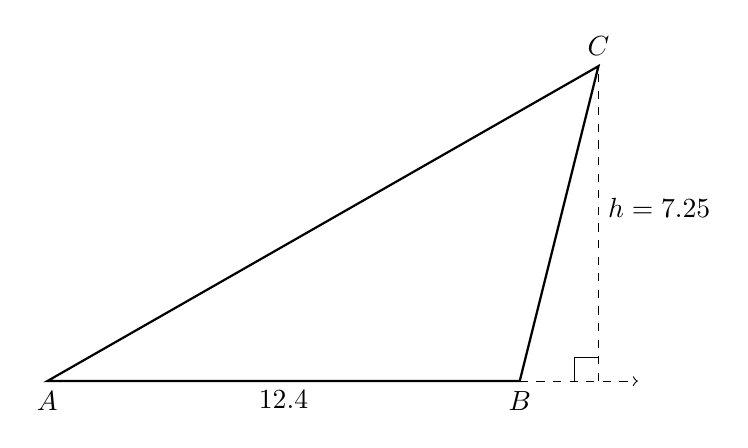
\begin{tikzpicture}[scale=1]
     \draw [thick]
       (0,0)node[below]{$A$}--
       (6,0)node[below]{$B$}--
       (7,4)node[above]{$C$} --cycle;
    \draw [dashed] (7,0)--(7,4);
    \draw [dashed, ->] (6,0)--(7.5,0);
    \draw (7,0)++(-0.3,0)--++(0,0.3)--+(0.3,0);
    \node at (7,2.2)[right]{$h=7.25$};
    \node at (3,0)[below]{$12.4$};
  \end{tikzpicture} \vspace{1.0cm}

\item Find the volume of a box (rectanglar prism) having a length of 8 centimeters, a depth of 4 cm, and a height of 5 cm. Show the calculation.
\begin{flushright}
  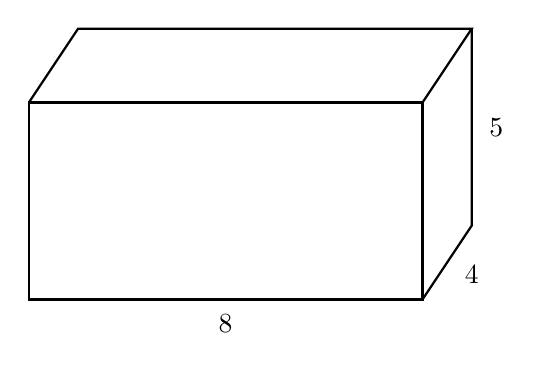
\begin{tikzpicture}[scale=1.25]
    \draw [-, thick] (0,0)--(4,0)--(4,2)--(0,2)--cycle;
    \draw [-, thick] (0,2)--(0.5,2.75)--(4.5,2.75)--(4,2);
    \draw [-, thick] (4,0)--(4.5,0.75)--(4.5,2.75);
    \node at (4.75, 1.75){$5$};
    \node at (2, -0.25){$8$};
    \node at (4.5, 0.25){$4$};
  \end{tikzpicture}
  \end{flushright} \vspace{2cm}  
  
\newpage
\item As shown below, two lines intersect making four angles: $\angle 1$, $\angle 2$, $\angle 3$, and $\angle 4$. Given that $m\angle 1= 4x+30$ and $m\angle 3=8x-10$, find $m\angle 1$. (check your solution)
    \begin{flushright}
    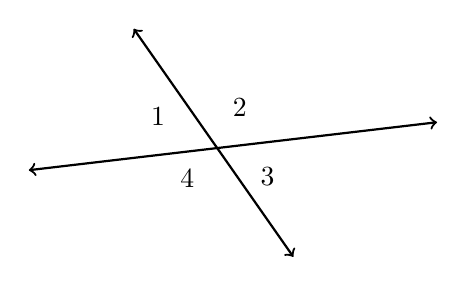
\begin{tikzpicture}[scale=0.5, rotate=-10]
      \draw [<->, thick] (0,-1.5)--(10,1.5);
      \draw [<->, thick] (2,2.5)--(7,-2.5);
      \node at (3,.4){1};
      \node at (6,-.6){3};
      \node at (5,1){2};
      \node at (4,-1){4};
      %\draw [fill] (0,0) circle [radius=0.05] node[below]{$P$};
      %\draw [fill] (6,0) circle [radius=0.05] node[below]{$R$};
      %\draw [fill] (3,0) circle [radius=0.05] node[below]{$Q$};
    \end{tikzpicture}
    \end{flushright} \vspace{2cm} 

\item The volume of the rectanglar prism shown is 80 cubic meters. Its length is 10 meters and depth 4 m. Find its height $h$. Show the calculation. (not drawn to scale)
\begin{flushright}
  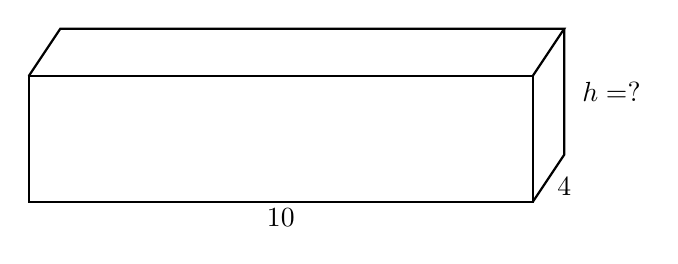
\begin{tikzpicture}[scale=0.8]
    \draw [-, thick] (0,0)--(8,0)--(8,2)--(0,2)--cycle;
    \draw [-, thick] (0,2)--(0.5,2.75)--(8.5,2.75)--(8,2);
    \draw [-, thick] (8,0)--(8.5,0.75)--(8.5,2.75);
    \node at (9.25, 1.75){$h=?$};
    \node at (4, -0.25){$10$};
    \node at (8.5, 0.25){$4$};
  \end{tikzpicture}
  \end{flushright} \vspace{1cm} 

\item The shape shown below is a trapezoid. Its height is 2 cm and the longer base is 8 cm. The shorter side opposite the base is 7 cm. \\[0.25cm]
Find the area of the trapezoid by adding the rectangular area to the triangle part.
\begin{flushright} 
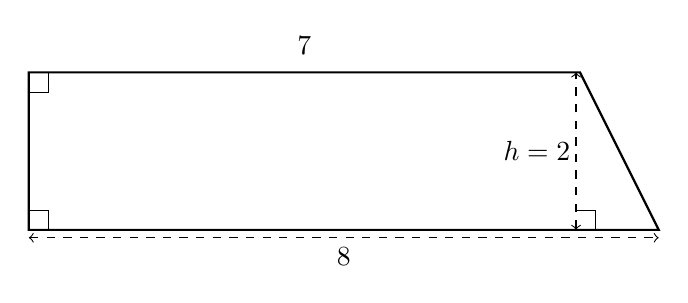
\begin{tikzpicture}[scale=1]
  \draw [thick]
  (0,0)--(0,2)--(7,2)--(8,0)--cycle;
  \draw [dashed,<->] (6.95,0)--(6.95,2);
  %\draw [dashed,<->] (0,2.1)--(7,2.1);
  %\draw [->] (45:0.5)--(45:0.9142);
  %\draw [->] (45:2.3)--(45:1.9142);
  \draw (0,0)++(0,0.25)--++(0.25,0)--+(0,-0.25);
  \draw (0,2)++(0,-0.25)--++(0.25,0)--+(0,0.25);
  \draw (6.95,0)++(0,0.25)--++(0.25,0)--+(0,-0.25);
  \draw [dashed,<->] (0,-0.1)--(8,-0.1);
  \node at (4,-0.1)[below]{$8$};
  \node at (7,1)[left]{$h=2$};
  \node at (3.5,2.1)[above]{$7$};
\end{tikzpicture}
\end{flushright} 
 \vspace{4cm}

\end{enumerate}
\end{document}